\documentclass[12pt,a4paper]{article}
\usepackage[a4paper, margin=0.8in, headheight=14pt]{geometry}
\usepackage{fontspec}
\usepackage{unicode-math}
\setmainfont{TeX Gyre Pagella}
\setmonofont[Scale=0.88]{TeX Gyre Cursor}
\setmathfont{Latin Modern Math}
\usepackage{xcolor}
\usepackage{colortbl}
\usepackage{titlesec}
\usepackage{enumitem}
\usepackage{tabularx}
\usepackage{booktabs}
\usepackage{array}
\usepackage{amsmath}
\usepackage{tikz}
\usetikzlibrary{shapes.geometric, arrows.meta, positioning, calc, fit, decorations.pathreplacing, decorations.pathmorphing}
\usepackage{tcolorbox}
\tcbuselibrary{skins, breakable}
\usepackage{hyperref}
\usepackage{fancyhdr}
\usepackage{graphicx}
\usepackage{microtype}
\hyphenpenalty=10000
\exhyphenpenalty=10000
\sloppy
\usepackage{caption}
\usepackage{setspace}
\usepackage{multirow}
\usepackage{tocloft}
\newcommand{\Q}[1]{\textbf{#1}\par\noindent\ignorespaces}
\definecolor{myred}{RGB}{196,30,58}
\definecolor{mydark}{RGB}{30,30,50}
\definecolor{mygreen}{RGB}{14,120,80}
\definecolor{myteal}{RGB}{0,130,140}
\definecolor{myamber}{RGB}{180,100,0}
\definecolor{mypurple}{RGB}{100,30,160}
\definecolor{mygray}{RGB}{246,247,249}
\definecolor{mgframe}{RGB}{180,185,200}
\definecolor{watermark}{RGB}{145,150,170}
\definecolor{hdrred}{RGB}{250,232,235}
\definecolor{hdrgreen}{RGB}{220,244,233}
\definecolor{hdrteal}{RGB}{220,242,244}
\definecolor{hdramber}{RGB}{253,242,215}
\definecolor{hdrpurple}{RGB}{238,228,255}
\definecolor{hdrgray}{RGB}{238,240,245}
\definecolor{rowalt}{RGB}{250,251,253}

\titleformat{\section}{\large\bfseries\color{myred}}{\thesection.}{0.5em}{}[\vspace{1pt}{\color{myred}\rule{\linewidth}{0.8pt}}]
\titleformat{\subsection}{\normalsize\bfseries\color{myteal}}{\thesubsection}{0.5em}{}
\titlespacing*{\section}{0pt}{18pt}{7pt}
\titlespacing*{\subsection}{0pt}{11pt}{4pt}
\setlength{\parindent}{0pt}
\setlength{\parskip}{4pt}
\renewcommand{\cfttoctitlefont}{\large\bfseries\color{myred}}
\renewcommand{\cftaftertoctitle}{\par\noindent{\color{myred}\rule{\linewidth}{0.8pt}}}
\setlength{\cftbeforetoctitleskip}{0pt}
\setlength{\cftaftertoctitleskip}{6pt}
\renewcommand{\cftsecfont}{\normalsize\bfseries\color{mydark}}
\renewcommand{\cftsecpagefont}{\normalsize\bfseries\color{mydark}}
\renewcommand{\cftsecleader}{\cftdotfill{\cftdotsep}}
\setlength{\cftbeforesecskip}{7pt}
\renewcommand{\cftsubsecfont}{\small\color{mydark}}
\renewcommand{\cftsubsecpagefont}{\small\color{mydark}}
\setlength{\cftbeforesubsecskip}{3pt}
\setlength{\cftsubsecindent}{1.4em}
\renewcommand{\cftpartfont}{\normalsize\bfseries\color{myteal}}
\renewcommand{\cftpartpagefont}{\normalsize\bfseries\color{myteal}}
\setlength{\cftbeforepartskip}{14pt}
\renewcommand{\arraystretch}{1.45}
\setlength{\tabcolsep}{6pt}
\arrayrulecolor{mydark}
\newcolumntype{B}[1]{>{\small\bfseries\raggedright\arraybackslash}m{#1}}
\newcolumntype{C}[1]{>{\centering\arraybackslash}m{#1}}
\newcolumntype{Y}{>{\small\raggedright\arraybackslash}X}
\renewcommand{\tabularxcolumn}[1]{m{#1}}
\newcommand{\currmodule}{Module 1}
\pagestyle{fancy}
\fancyhf{}
\fancyhead[L]{\small\color{myred}\textbf{OE-EC704B}\;\color{mydark}--- Optimization Technique}
\fancyhead[R]{\small\color{myteal}\textbf{\currmodule\ Notes}}
\fancyfoot[C]{\small\color{mydark}\thepage}
\fancyfoot[R]{\small\color{watermark}\textit{\copyright\ Biraj}}
\renewcommand{\headrulewidth}{0.5pt}
\renewcommand{\footrulewidth}{0.3pt}

\hypersetup{colorlinks=true, linkcolor=myteal, urlcolor=myteal,
  pdfauthor={Biraj Sarkar},
  pdftitle={OE-EC704B --- Combined Notes}}

\tcbset{
  tikzbox/.style={
    colback=mygray, colframe=mgframe, boxrule=0.6pt, arc=4pt,
    left=8pt, right=8pt, top=6pt, bottom=6pt,
    colbacktitle=mgframe, coltitle=mydark,
    fonttitle=\small\bfseries
  },
  defbox/.style={
    colback=hdrgreen, colframe=mygreen, boxrule=0.8pt, arc=4pt,
    left=9pt, right=9pt, top=6pt, bottom=6pt,
    colbacktitle=mygreen, coltitle=white,
    fonttitle=\small\bfseries
  },
  formulabox/.style={
    colback=hdrteal, colframe=myteal, boxrule=0.8pt, arc=4pt,
    left=9pt, right=9pt, top=7pt, bottom=7pt,
    colbacktitle=myteal, coltitle=white,
    fonttitle=\small\bfseries
  },
  examplebox/.style={
    colback=hdramber, colframe=myamber, boxrule=0.8pt, arc=4pt,
    left=9pt, right=9pt, top=6pt, bottom=6pt,
    colbacktitle=myamber, coltitle=white,
    fonttitle=\small\bfseries
  },
  masonbox/.style={
    colback=hdrpurple, colframe=mypurple, boxrule=0.8pt, arc=4pt,
    left=9pt, right=9pt, top=6pt, bottom=6pt,
    colbacktitle=mypurple, coltitle=white,
    fonttitle=\small\bfseries
  },
  exambox/.style={
    colback=hdrpurple, colframe=mypurple, boxrule=1pt, arc=5pt,
    left=10pt, right=10pt, top=8pt, bottom=8pt,
    colbacktitle=mypurple, coltitle=white,
    fonttitle=\bfseries,
    breakable, title after break={\textbf{Frequently Asked / Viva Questions (contd.)}}}
}
\tcbset{breakable}
\tcbset{after={\color{black}}}

\tikzset{
  block/.style={rectangle, draw=myteal, fill=hdrteal,
    text width=2.4cm, align=center, minimum height=0.95cm,
    font=\small, rounded corners=3pt, line width=0.7pt},
  redblock/.style={rectangle, draw=myred, fill=hdrred,
    text width=2.4cm, align=center, minimum height=0.95cm,
    font=\small, rounded corners=3pt, line width=0.7pt},
  netnode/.style={rectangle, draw=myteal, fill=hdrteal,
    text width=1.5cm, align=center, minimum height=0.8cm,
    font=\small, rounded corners=3pt, line width=0.7pt},
  sumjunc/.style={circle, draw=myamber, fill=hdramber,
    minimum size=0.62cm, font=\small, line width=0.8pt},
  snode/.style={circle, draw=mypurple, fill=hdrpurple,
    minimum size=0.55cm, font=\footnotesize, line width=0.7pt},
  arrow/.style={-Stealth, thick, color=mydark},
  redarrow/.style={-Stealth, thick, color=myred},
  line/.style={thick, color=mydark}
}

\newcommand{\modulestart}[2]{%
  \clearpage
  \renewcommand{\currmodule}{Module #1}%
  \renewcommand{\theHsection}{mod#1.\arabic{section}}%
  \renewcommand{\theHsubsection}{\theHsection.\arabic{subsection}}%
  \renewcommand{\theHsubsubsection}{\theHsubsection.\arabic{subsubsection}}%
  \phantomsection
  \addcontentsline{toc}{part}{Module #1: #2}%
  \setcounter{section}{0}%
  \begin{center}
    \vspace*{1.0cm}
    {\Huge\bfseries\color{myred} Module #1}\\[10pt]
    {\Large\bfseries\color{mydark} #2}\\[10pt]
    {\color{myred}\rule{0.55\linewidth}{1.2pt}}
  \end{center}
  \vspace{14pt}
}
\begin{document}

\thispagestyle{empty}
\vspace*{1.0cm}
\begin{center}
  {\Huge\bfseries\color{myred} OE-EC704B}\\[10pt]
  {\LARGE\bfseries\color{mydark} Optimization Technique}\\[20pt]
  {\color{myred}\rule{0.7\linewidth}{1.5pt}}\\[18pt]
  {\Large\color{myteal}\textbf{Combined Module Notes}}\\[8pt]
  {\large\color{mydark} Modules 1 -- 6}\\[40pt]
  {\normalsize\color{mydark} Semester VII \quad$\bullet$\quad 3L:0T:0P \quad$\bullet$\quad 3 Credits}\\[12pt]
  {\normalsize\color{mydark} CGEC \;$|$\; B.Tech ECE (2023--27)}\\[6pt]
  {\normalsize\color{mydark}\textit{Biraj Sarkar}}
\end{center}
\vspace{1.0cm}
\begin{center}
  \begin{tcolorbox}[colback=mygray, colframe=mgframe, boxrule=0.5pt, arc=3pt, width=0.85\linewidth]
    \centering\small\color{mydark}
    \textbf{Disclaimer / Study Guide Notice:}\\
    These are condensed \textbf{Short Notes} focusing on core theory, key formulas, block/circuit diagrams, and standard viva Q\&As for university exam revision. Exhaustive numerical practice problems and derivation edge cases are not covered. This serves as a quick-revision reference guide for students.
  \end{tcolorbox}
\end{center}
\vfill
\begin{center}{\small\color{watermark}\textit{Exam-Ready Notes}}\end{center}
\clearpage

\hypersetup{linkcolor=mydark}
\tableofcontents
\hypersetup{linkcolor=myteal}
\clearpage

% -- Module 1 -----------------------------------------------------------------
\modulestart{1}{Introduction to Optimization}

\section{Introduction to Optimization}
% ===============================================================================

Optimization is the act of obtaining the best result under given circumstances. In engineering design, it refers to making decisions that maximize desired factors (such as efficiency, reliability, or strength) or minimize undesired factors (such as cost, weight, or energy loss).

\subsection{Standard Mathematical Formulation}
Every optimization problem can be formulated in a canonical mathematical representation:

\begin{tcolorbox}[defbox, title={Canonical Optimization Problem}]
Minimize the objective function:
\begin{equation}
  f(\mathbf{x}) = f(x_1, x_2, \dots, x_n)
\end{equation}
subject to:
\begin{align}
  g_j(\mathbf{x}) &\le 0, \quad j = 1, 2, \dots, m \quad \text{(Inequality Constraints)} \\
  h_k(\mathbf{x}) &= 0, \quad k = 1, 2, \dots, p \quad \text{(Equality Constraints)}
\end{align}
and the variable bounds (side constraints):
\begin{equation}
  x_i^{(L)} \le x_i \le x_i^{(U)}, \quad i = 1, 2, \dots, n
\end{equation}
Where $\mathbf{x} = [x_1, x_2, \dots, x_n]^T$ is the design vector.
\end{tcolorbox}

\subsection{Key Design Elements}
\begin{enumerate}[label=\textbf{\arabic*.}, leftmargin=*, itemsep=4pt]
  \item \textbf{Design Vector (\texorpdfstring{$\mathbf{x}$}{x}):} A set of $n$ independent variables that uniquely define the design. These parameters are varied by the optimizer (e.g., length, thickness, resistance, voltage).
  \item \textbf{Objective Function (\texorpdfstring{$f(\mathbf{x})$}{f(x)}):} A mathematical expression that quantifies the criterion to be optimized. If the objective is maximization, it is equivalent to minimizing $-f(\mathbf{x})$.
  \item \textbf{Design Constraints:} Conditions that must be satisfied for a design to be acceptable.
    \begin{itemize}[label=\tiny$\bullet$, leftmargin=1.5em, itemsep=2pt]
      \item \textit{Behavior Constraints:} Restraints on the functional behavior of the system (e.g., max deflection, voltage limit).
      \item \textit{Geometric / Side Constraints:} Direct limits on physical dimensions (e.g., thickness $t \ge 2\text{ mm}$).
    \end{itemize}
  \item \textbf{Feasible Region:} The set of all design points in the design space that satisfy all equality and inequality constraints.
\end{enumerate}

% ===============================================================================
\section{Engineering Optimization Problem Formulation}
% ===============================================================================

To optimize an engineering system, the physical problem must be translated into standard mathematical form.

\subsection{Classic Example: Design of a Cylindrical Water Tank}
Let us formulate the problem of designing a cylindrical water tank of a specified storage capacity ($V_0$) that minimizes the total manufacturing cost (material cost).

\begin{tcolorbox}[examplebox, title={Cylindrical Tank Optimization Formulation}]
\textbf{1. Design Variables:}
Let the radius of the tank be $r$ and the height be $h$.
\begin{equation*}
  \mathbf{x} = [r, h]^T
\end{equation*}

\textbf{2. Objective Function:}
To minimize the manufacturing cost, we minimize the total surface area (base area + cylindrical wall area):
\begin{equation}
  \text{Minimize } f(r, h) = \pi r^2 + 2\pi r h
\end{equation}

\textbf{3. Constraints:}
The tank must hold a minimum volume $V_0$:
\begin{equation*}
  \pi r^2 h \ge V_0 \implies V_0 - \pi r^2 h \le 0
\end{equation*}
Hence, the inequality constraint is:
\begin{equation}
  g_1(r, h) = V_0 - \pi r^2 h \le 0
\end{equation}
Additionally, we have non-negativity side constraints:
\begin{equation}
  r \ge 0, \quad h \ge 0
\end{equation}
\end{tcolorbox}

% ===============================================================================
\section{Classification of Optimization Problems}
% ===============================================================================

Optimization problems are classified based on structure, constraints, and objective behaviors:

\par\noindent
{\renewcommand{\arraystretch}{1.5}%
\begin{tabularx}{\linewidth}{|B{3.2cm}|Y|Y|}\hline
\multicolumn{1}{|>{\centering\arraybackslash}m{3.2cm}|}{\textbf{Parameter}} &
\multicolumn{1}{>{\centering\arraybackslash}Y|}{\textbf{Class A}} &
\multicolumn{1}{>{\centering\arraybackslash}Y|}{\textbf{Class B}} \\
\hline
\textbf{Constraints} & \textbf{Unconstrained:} No limits on design space; $\min f(\mathbf{x})$. & \textbf{Constrained:} Limits exist ($g_j(\mathbf{x}) \le 0$, $h_k(\mathbf{x}) = 0$). \\
\hline
\textbf{Linearity} & \textbf{Linear Programming (LP):} $f$, $g_j$, and $h_k$ are all linear functions of $\mathbf{x}$. & \textbf{Non-linear Programming (NLP):} At least one function is non-linear. \\
\hline
\textbf{Variables} & \textbf{Single-variable:} $f(x)$ depends on one parameter only. & \textbf{Multivariable:} $f(\mathbf{x})$ depends on two or more parameters. \\
\hline
\textbf{Nature} & \textbf{Static:} Design variables represent constant parameters. & \textbf{Dynamic:} Design variables are functions of time. \\
\hline
\end{tabularx}
}

% ===============================================================================
\section{Classification of Optimization Algorithms}
% ===============================================================================

Optimization algorithms are structured into three primary groups based on search logic:

\begin{enumerate}[label=\textbf{\Roman*.}, leftmargin=*, itemsep=4pt]
  \item \textbf{Analytical Methods (Calculus-Based):} Uses derivative information ($f'(x)$, $\nabla f$) to establish optimality conditions. Extremely fast but requires the objective function to be continuous and differentiable.
  \item \textbf{Numerical Methods (Search-Based):} Iterative procedures that evaluate the objective function at sequence points to narrow down the optimum.
    \begin{itemize}[label=\tiny$\bullet$, leftmargin=1.5em, itemsep=2pt]
      \item \textit{Direct Search Methods:} Require objective function values only (e.g., Simplex, Hooke-Jeeves).
      \item \textit{Gradient-Based Methods:} Require function value and derivative values (e.g., Steepest Descent, Newton).
    \end{itemize}
  \item \textbf{Advanced / Meta-heuristic Algorithms:} Nature-inspired algorithms that explore global design spaces to bypass local minima traps (e.g., Genetic Algorithms, Particle Swarm Optimization, Simulated Annealing).
\end{enumerate}

\subsection{The Optimization Design Loop}
The sequence of engineering design optimization is mapped below:

\begin{tcolorbox}[tikzbox, title={Optimization Design Process Flowchart}]
\centering
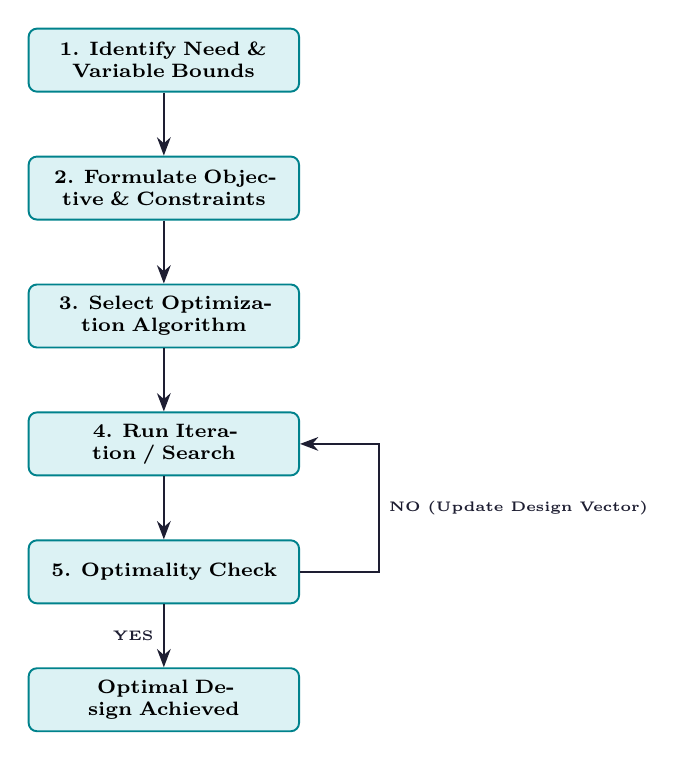
\begin{tikzpicture}[
  node distance=0.8cm and 1.5cm,
  block/.style={rectangle, draw=myteal, fill=hdrteal, text width=3.2cm, align=center, minimum height=0.8cm, font=\scriptsize\bfseries, rounded corners=3pt, line width=0.7pt},
  arrow/.style={-Stealth, thick, color=mydark}
]
  \node[block] (s1) {1. Identify Need \& Variable Bounds};
  \node[block, below=of s1] (s2) {2. Formulate Objective \& Constraints};
  \node[block, below=of s2] (s3) {3. Select Optimization Algorithm};
  \node[block, below=of s3] (s4) {4. Run Iteration / Search};
  \node[block, below=of s4] (s5) {5. Optimality Check};
  \node[block, below=of s5] (s6) {Optimal Design Achieved};

  \draw[arrow] (s1) -- (s2);
  \draw[arrow] (s2) -- (s3);
  \draw[arrow] (s3) -- (s4);
  \draw[arrow] (s4) -- (s5);
  \draw[arrow] (s5) -- node[left, font=\tiny\bfseries\color{mygreen}] {YES} (s6);
  
  \draw[arrow] (s5.east) -- ++(1.0,0) |- node[pos=0.25, right, font=\tiny\bfseries\color{myred}] {NO (Update Design Vector)} (s4.east);
\end{tikzpicture}
\end{tcolorbox}

\newpage

% ===============================================================================
% MANDATORY QUICK REVISION PAGE
% ===============================================================================
\begin{center}
  {\large\bfseries\color{myred} Quick Revision --- Module 1}\\[3pt]
  {\small\color{mydark} Mathematical Formulation \& Fundamentals $|$ OE-EC704B}
\end{center}
\noindent{\color{myred}\rule{\linewidth}{1.2pt}}
\vspace{4pt}

\begin{tcolorbox}[formulabox, title={\textbf{Key Concepts \& Mathematical Rules}}]
\renewcommand{\arraystretch}{1.35}
\begin{tabularx}{\linewidth}{B{5.0cm} X}
Objective Function & $f(\mathbf{x}) \rightarrow$ function to be minimized or maximized. \\[4pt]
Inequality Constraints & $g_j(\mathbf{x}) \le 0, \quad j=1,\dots,m$. \\[4pt]
Equality Constraints & $h_k(\mathbf{x}) = 0, \quad k=1,\dots,p$. \\[4pt]
Side Constraints & $x_i^{(L)} \le x_i \le x_i^{(U)}, \quad i=1,\dots,n$. \\[4pt]
Design Vector & $\mathbf{x} = [x_1, x_2, \dots, x_n]^T$ containing $n$ design variables. \\
\end{tabularx}
\end{tcolorbox}

\begin{tcolorbox}[defbox, title={\textbf{One-Line Definitions}}]
\begin{itemize}[leftmargin=*, itemsep=2.5pt, topsep=0pt]
  \item \textbf{Design Variable:} An independent parameter that can be varied during the design optimization process.
  \item \textbf{Behavior Constraint:} A constraint bounding the system behavior under operational loads (e.g., maximum stress).
  \item \textbf{Feasible Space:} The region of design space in which all inequality and equality constraints are fully satisfied.
  \item \textbf{Non-linear Programming (NLP):} An optimization problem containing non-linearities in objective or constraint functions.
  \item \textbf{Global Minimum:} The absolute lowest value of the objective function in the entire feasible design space.
  \item \textbf{Local Minimum:} The lowest value of the objective function within a local neighborhood of the design space.
\end{itemize}
\end{tcolorbox}

\begin{tcolorbox}[exambox, title={\textbf{Frequently Asked / Viva Questions}}]
\begin{enumerate}[topsep=0pt, label=\textbf{Q\arabic*.}, itemsep=5pt]
  \item \Q{State the standard mathematical formulation of a constrained optimization problem.}
    Minimize $f(\mathbf{x})$ subject to $g_j(\mathbf{x}) \le 0$ for $j=1,\dots,m$, $h_k(\mathbf{x}) = 0$ for $k=1,\dots,p$, and $x_i^{(L)} \le x_i \le x_i^{(U)}$ for $i=1,\dots,n$.
  \item \Q{Differentiate between design variables and design parameters.}
    Design variables are changed by the optimization algorithm to find the optimum design. Design parameters are constant coefficients fixed before the optimization starts (e.g., material density, young's modulus).
  \item \Q{Differentiate between behavior constraints and side constraints.}
    Behavior constraints depend on the state variables of the system and require system analysis to evaluate (e.g., stress $\le \sigma_{allow}$). Side constraints directly bound the design variables (e.g., diameter $d \ge 10\text{ mm}$).
  \item \Q{What is a feasible design space?}
    A feasible design space is the collection of all design vectors $\mathbf{x}$ that satisfy all constraints simultaneously.
  \item \Q{What is the difference between single-objective and multi-objective optimization?}
    Single-objective optimization seeks to optimize a single criterion. Multi-objective optimization optimizes multiple conflicting objectives simultaneously, yielding a set of trade-off designs (Pareto front).
  \item \Q{Why do we reformulate a maximization problem as a minimization problem?}
    To maintain algorithmic consistency. Any maximization problem can be solved using standard minimization algorithms by minimizing $-f(\mathbf{x})$.
  \item \Q{What makes a problem a Linear Programming Problem (LPP)?}
    An optimization problem is an LPP if the objective function and all equality/inequality constraints are linear functions of the design variables.
  \item \Q{Classify optimization methods based on their search logic.}
    Methods are classified into Analytical Methods (calculus-based), Numerical Methods (Search-based: Direct and Gradient-based), and Advanced Heuristic Methods (nature-inspired: GA, PSO, SA).
  \item \Q{Explain the role of the objective function.}
    The objective function acts as a mathematical evaluator that measures how good a particular candidate design vector is relative to design goals.
  \item \Q{What are the side constraints in cylinder volume maximization under surface area limits?}
    The side constraints are the physical non-negativity limits of the geometric parameters: Radius $r \ge 0$ and Height $h \ge 0$.
\end{enumerate}
\end{tcolorbox}


% -- Module 2 -----------------------------------------------------------------
\modulestart{2}{Optimality Criteria for Single-Variable Functions}

\section{Optimality Criteria for Single-Variable Functions}
% ===============================================================================

Optimality criteria determine whether a candidate point $x^*$ is a local minimum, local maximum, or an inflection point.

\subsection{Necessary Condition (First-Order)}
\begin{tcolorbox}[defbox, title={Theorem: Necessary Condition}]
If a function $f(x)$ is continuous and differentiable at $x^*$, and $x^*$ is a local extremum (minimum or maximum), then the first derivative at $x^*$ must vanish:
\begin{equation}
  f'(x^*) = \left. \frac{df}{dx} \right|_{x = x^*} = 0
\end{equation}
Such a point $x^*$ is called a \textbf{Stationary Point}.
\end{tcolorbox}

\subsection{Sufficient Condition (Second-Order)}
\begin{tcolorbox}[defbox, title={Theorem: Sufficient Condition}]
Let $f(x)$ be twice differentiable at the stationary point $x^*$.
\begin{itemize}[leftmargin=*, itemsep=2pt, topsep=0pt]
  \item If $f''(x^*) > 0$, then $x^*$ is a \textbf{local minimum}.
  \item If $f''(x^*) < 0$, then $x^*$ is a \textbf{local maximum}.
  \item If $f''(x^*) = 0$, the test is inconclusive. We must evaluate higher-order derivatives:
    \begin{equation}
      f'(x^*) = f''(x^*) = \dots = f^{(n-1)}(x^*) = 0, \quad f^{(n)}(x^*) \neq 0
    \end{equation}
    \begin{itemize}[label=\tiny$\bullet$, leftmargin=1.5em, itemsep=1.5pt]
      \item If $n$ is \textbf{odd}, $x^*$ is an \textbf{inflection point} (neither minimum nor maximum).
      \item If $n$ is \textbf{even} and $f^{(n)}(x^*) > 0$, $x^*$ is a \textbf{local minimum}.
      \item If $n$ is \textbf{even} and $f^{(n)}(x^*) < 0$, $x^*$ is a \textbf{local maximum}.
    \end{itemize}
\end{itemize}
\end{tcolorbox}

% ===============================================================================
\section{Bracketing Methods}
% ===============================================================================

Bracketing methods find an initial interval of uncertainty containing the optimum before applying fast search routines.

\subsection{Exhaustive Search Method}
Exhaustive search evaluates a function at equally spaced points in an interval $[a, b]$ to find the sub-interval containing the minimum.

\begin{tcolorbox}[formulabox, title={Exhaustive Search Algorithm}]
Let the initial interval be $[a, b]$, and let the number of evaluations be $n$.
\begin{enumerate}[label=\textbf{\arabic*.}, leftmargin=*, itemsep=2pt, topsep=0pt]
  \item Calculate the step size:
    \begin{equation}
      \Delta x = \frac{b - a}{n}
    \end{equation}
  \item Define evaluation coordinates: $x_i = a + i \cdot \Delta x$, for $i = 0, 1, \dots, n$.
  \item Evaluate $f(x_i)$ sequentially for $i = 1, 2, \dots, n-1$.
  \item Identify three consecutive points $x_{k-1}$, $x_k$, and $x_{k+1}$ such that:
    \begin{equation}
      f(x_{k-1}) > f(x_k) \quad \text{and} \quad f(x_k) < f(x_{k+1})
    \end{equation}
  \item The minimum lies bracketed in the interval $[x_{k-1}, x_{k+1}]$. The new interval of uncertainty is:
    \begin{equation}
      L_1 = 2 \cdot \Delta x = \frac{2(b - a)}{n}
    \end{equation}
\end{enumerate}
\end{tcolorbox}

% ===============================================================================
\section{Region-Elimination Methods}
% ===============================================================================

Region-elimination methods systematically reduce the interval of uncertainty by comparing objective values at test points.

\subsection{Working Principle of Region Elimination}
If we assume $f(x)$ is \textbf{unimodal} (has only one minimum in the interval $[a, b]$), we can eliminate a portion of the interval by evaluating two test points $x_1$ and $x_2$ (where $x_1 < x_2$):

\begin{tcolorbox}[tikzbox, title={Unimodal Region Elimination Logic}]
\centering
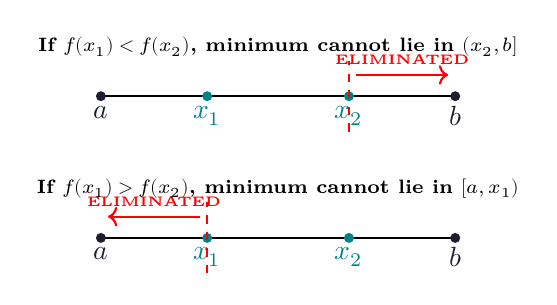
\begin{tikzpicture}[scale=0.9]
  % Case 1: f(x1) < f(x2)
  \draw[thick] (0,0) -- (5,0);
  \fill[mydark] (0,0) circle (2pt) node[below] {$a$};
  \fill[mydark] (5,0) circle (2pt) node[below] {$b$};
  \fill[myteal] (1.5,0) circle (2pt) node[below] {$x_1$};
  \fill[myteal] (3.5,0) circle (2pt) node[below] {$x_2$};
  \draw[dashed, red, thick] (3.5,-0.5) -- (3.5,0.5);
  \draw[red, ->, thick] (3.6, 0.3) -- (4.9, 0.3) node[midway, above, font=\tiny\bfseries] {ELIMINATED};
  \node[font=\scriptsize\bfseries] at (2.5, 0.7) {If $f(x_1) < f(x_2)$, minimum cannot lie in $(x_2, b]$};

  % Case 2: f(x1) > f(x2)
  \begin{scope}[yshift=-2.0cm]
    \draw[thick] (0,0) -- (5,0);
    \fill[mydark] (0,0) circle (2pt) node[below] {$a$};
    \fill[mydark] (5,0) circle (2pt) node[below] {$b$};
    \fill[myteal] (1.5,0) circle (2pt) node[below] {$x_1$};
    \fill[myteal] (3.5,0) circle (2pt) node[below] {$x_2$};
    \draw[dashed, red, thick] (1.5,-0.5) -- (1.5,0.5);
    \draw[red, ->, thick] (1.4, 0.3) -- (0.1, 0.3) node[midway, above, font=\tiny\bfseries] {ELIMINATED};
    \node[font=\scriptsize\bfseries] at (2.5, 0.7) {If $f(x_1) > f(x_2)$, minimum cannot lie in $[a, x_1)$};
  \end{scope}
\end{tikzpicture}
\end{tcolorbox}

\subsection{Interval Halving Method}
This method eliminates exactly half of the interval at each stage using three evaluations ($x_0$, $x_1$, and $x_2$).

\begin{tcolorbox}[formulabox, title={Interval Halving Algorithm}]
Let the current interval be $[a, b]$.
\begin{enumerate}[label=\textbf{\arabic*.}, leftmargin=*, itemsep=2pt, topsep=0pt]
  \item Calculate the midpoint: $x_0 = \frac{a+b}{2}$.
  \item Calculate quarter points:
    \begin{equation}
      x_1 = a + \frac{b-a}{4}, \quad x_2 = b - \frac{b-a}{4}
    \end{equation}
  \item Evaluate $f(x_1)$, $f(x_0)$, and $f(x_2)$.
  \item Compare function values to eliminate region:
    \begin{itemize}[label=\tiny$\bullet$, leftmargin=1.5em, itemsep=1.5pt]
      \item If $f(x_1) < f(x_0)$, the new interval is $[a, x_0]$.
      \item If $f(x_2) < f(x_0)$, the new interval is $[x_0, b]$.
      \item If $f(x_1) \ge f(x_0)$ and $f(x_2) \ge f(x_0)$, the new interval is $[x_1, x_2]$.
    \end{itemize}
  \item In all cases, the new interval width is exactly:
    \begin{equation}
      L_{new} = \frac{b-a}{2}
    \end{equation}
\end{enumerate}
\end{tcolorbox}

\subsection{Fibonacci Search Method}
Fibonacci search is the mathematically optimal region-elimination method. It uses the Fibonacci sequence $F_0 = 1$, $F_1 = 1$, $F_n = F_{n-1} + F_{n-2}$ to calculate placement ratios.

\begin{tcolorbox}[formulabox, title={Fibonacci Search Equations}]
For a pre-selected total number of function evaluations $n$:
\begin{enumerate}[label=\textbf{\arabic*.}, leftmargin=*, itemsep=3pt, topsep=0pt]
  \item The initial two test points $x_1$ and $x_2$ in $[a, b]$ are placed at:
    \begin{equation}
      x_1 = a + \frac{F_{n-2}}{F_n}(b - a)
    \end{equation}
    \begin{equation}
      x_2 = b - \frac{F_{n-2}}{F_n}(b - a) = a + \frac{F_{n-1}}{F_n}(b - a)
    \end{equation}
  \item After region elimination, the remaining sub-interval is evaluated. At the $k$-th step, the new test point is placed at:
    \begin{equation}
      x_k = \text{Remaining Limit} \pm \frac{F_{n-k-1}}{F_{n-k+1}}(\text{Current Interval Width})
    \end{equation}
  \item The final reduction ratio of the interval of uncertainty after $n$ iterations is:
    \begin{equation}
      \frac{L_n}{L_1} = \frac{1}{F_n}
    \end{equation}
\end{enumerate}
\end{tcolorbox}

% ===============================================================================
\section{Point Estimation Methods}
% ===============================================================================

Unlike region elimination, point estimation methods fit a smooth polynomial through known points to estimate the local minimum directly.

\subsection{Successive Quadratic Estimation (SQE)}
SQE fits a quadratic function $q(x) = A x^2 + B x + C$ through three test points $x_1 < x_2 < x_3$ with known function values $f_1, f_2, f_3$.

\begin{tcolorbox}[formulabox, title={SQE Minimum Point Formula}]
The minimum $x^*$ of the approximating quadratic polynomial is given by:
\begin{equation}
  x^* = \frac{1}{2} \frac{(x_2^2 - x_3^2)f_1 + (x_3^2 - x_1^2)f_2 + (x_1^2 - x_2^2)f_3}{(x_2 - x_3)f_1 + (x_3 - x_1)f_2 + (x_1 - x_2)f_3}
\end{equation}
\par\vspace{3pt}
Alternatively, we can express the calculation using coordinate differences:
\begin{equation}
  x^* = x_2 + \frac{1}{2} \frac{(x_2 - x_1)^2(f_2 - f_3) - (x_2 - x_3)^2(f_2 - f_1)}{(x_2 - x_1)(f_2 - f_3) - (x_2 - x_3)(f_2 - f_1)}
\end{equation}
If $x^*$ is close to $x_2$ within a tolerance limit, $x^*$ is taken as the optimum. Otherwise, the worst point among $\{x_1, x_2, x_3\}$ is replaced by $x^*$, and the calculation is repeated.
\end{tcolorbox}

\newpage

% ===============================================================================
% MANDATORY QUICK REVISION PAGE
% ===============================================================================
\begin{center}
  {\large\bfseries\color{myred} Quick Revision --- Module 2}\\[3pt]
  {\small\color{mydark} Single-Variable Optimization $|$ OE-EC704B}
\end{center}
\noindent{\color{myred}\rule{\linewidth}{1.2pt}}
\vspace{4pt}

\begin{tcolorbox}[formulabox, title={\textbf{Key Formulas \& Equations}}]
\renewcommand{\arraystretch}{1.45}
\begin{tabularx}{\linewidth}{B{5.0cm} X}
Necessary Condition & $f'(x^*) = 0$ \quad (stationary point requirement). \\[4pt]
Sufficient Condition & $f''(x^*) > 0 \implies \text{local min}$; $f''(x^*) < 0 \implies \text{local max}$. \\[4pt]
Interval Halving Width & $L_{new} = \frac{1}{2} L_{old}$ \quad (achieved with 3 evaluations). \\[4pt]
Fibonacci Point 1 & $x_1 = a + \frac{F_{n-2}}{F_n}(b-a)$. \\[4pt]
Fibonacci Reduction Ratio & $\frac{L_n}{L_1} = \frac{1}{F_n}$ \quad (where $F_n$ is the $n$-th Fibonacci number). \\[4pt]
SQE Minimum Point & $x^* = x_2 + \frac{1}{2} \frac{(x_2 - x_1)^2(f_2 - f_3) - (x_2 - x_3)^2(f_2 - f_1)}{(x_2 - x_1)(f_2 - f_3) - (x_2 - x_3)(f_2 - f_1)}$. \\
\end{tabularx}
\end{tcolorbox}

\begin{tcolorbox}[defbox, title={\textbf{One-Line Definitions}}]
\begin{itemize}[leftmargin=*, itemsep=2.5pt, topsep=0pt]
  \item \textbf{Stationary Point:} A point at which the first derivative of a differentiable function is zero.
  \item \textbf{Inflection Point:} A point on a curve at which the concavity changes, where $f''(x)=0$ and $f'''(x) \neq 0$.
  \item \textbf{Unimodal Function:} A function that has exactly one local extremum (minimum or maximum) in a given interval.
  \item \textbf{Bracketing Method:} A search algorithm designed to find an initial interval containing the optimum.
  \item \textbf{Region Elimination:} Systematically discarding a sub-interval of search space using unimodality comparisons.
  \item \textbf{Fibonacci Search:} An optimal region-elimination search algorithm utilizing Fibonacci ratios.
  \item \textbf{Successive Quadratic Estimation:} An interpolation algorithm that fits quadratic curves through test coordinates to locate the minimum.
\end{itemize}
\end{tcolorbox}

\begin{tcolorbox}[exambox, title={\textbf{Frequently Asked / Viva Questions}}]
\begin{enumerate}[topsep=0pt, label=\textbf{Q\arabic*.}, itemsep=5pt]
  \item \Q{State the necessary and sufficient conditions for a local minimum of a single-variable function.}
    Necessary condition: $f'(x^*) = 0$. Sufficient condition: $f''(x^*) > 0$.
  \item \Q{What happens if $f'(x^*) = f''(x^*) = 0$ at a candidate point?}
    The test is inconclusive. We must evaluate higher-order derivatives. If the first non-zero derivative is of odd order, it is an inflection point. If it is of even order and positive, it is a local minimum.
  \item \Q{Define a unimodal function and state why it is important for region-elimination methods.}
    A function is unimodal if it has only one optimum in a given range. Unimodality guarantees that comparing function values at two points ($f(x_1)$ and $f(x_2)$) yields a valid sub-region to eliminate.
  \item \Q{How does the Interval Halving method work?}
    It divides the interval into four equal parts using three points ($x_1 < x_0 < x_2$). Comparing their function values allows the elimination of half the interval ($L_{new} = 0.5 L_{old}$).
  \item \Q{Why is the Fibonacci search method considered optimal among region-elimination techniques?}
    For a pre-specified number of evaluations $n$, it achieves the maximum possible reduction in the interval of uncertainty ($1/F_n$) without requiring any derivative information.
  \item \Q{What is the relation between Fibonacci search and Golden Section search?}
    Golden Section search is the limiting case of Fibonacci search as the number of evaluations $n \to \infty$. It uses the constant Golden Ratio $\gamma \approx 0.618$ instead of discrete Fibonacci fractions.
  \item \Q{Write down the quadratic estimation formula for the minimum point $x^*$.}
    $x^* = \frac{1}{2} \frac{(x_2^2 - x_3^2)f_1 + (x_3^2 - x_1^2)f_2 + (x_1^2 - x_2^2)f_3}{(x_2 - x_3)f_1 + (x_3 - x_1)f_2 + (x_1 - x_2)f_3}$ for three ordered points $x_1 < x_2 < x_3$.
  \item \Q{Differentiate between bracketing methods and point estimation methods.}
    Bracketing methods find an interval containing the optimum (e.g., Exhaustive Search). Point estimation methods fit functional approximations (e.g., quadratic curves) to predict the exact coordinate of the optimum.
  \item \Q{Under what conditions does the successive quadratic estimation (SQE) method converge?}
    SQE converges rapidly if the objective function is smooth, continuous, and has a unimodal shape resembling a parabola in the neighborhood of the optimum.
  \item \Q{What is the significance of the Fibonacci numbers sequence in search algorithms?}
    The Fibonacci numbers satisfy the property $F_{n-2}/F_n \to 0.382$ and $F_{n-1}/F_n \to 0.618$, which balances the spacing of evaluation points so that previous calculations are reused in subsequent steps.
\end{enumerate}
\end{tcolorbox}


% -- Module 3 -----------------------------------------------------------------
\modulestart{3}{Fundamentals of Gradient-Based Search}

\section{Fundamentals of Gradient-Based Search}
% ===============================================================================

Gradient-based single-variable methods use derivative information to find stationary points by solving:
\begin{equation}
  g(x) = f'(x) = 0
\end{equation}
These algorithms are highly efficient because derivatives provide the slope and curvature of the objective function, indicating the direction and distance to the optimum.

% ===============================================================================
\section{Newton-Raphson Method}
% ===============================================================================

The Newton-Raphson method is a second-order method that approximates the function locally with a quadratic Taylor series expansion.

\subsection{Derivation of the Iterative Formula}
Let $x_k$ be the current estimate of the optimum. Expanding the first derivative $f'(x)$ about $x_k$ using a first-order Taylor series yields:
\begin{equation*}
  f'(x) \approx f'(x_k) + f''(x_k)(x - x_k)
\end{equation*}
To locate the stationary point ($x_{k+1}$ where $f'(x_{k+1}) = 0$):
\begin{equation*}
  f'(x_k) + f''(x_k)(x_{k+1} - x_k) = 0
\end{equation*}
Rearranging for $x_{k+1}$ gives the standard \textbf{Newton-Raphson Update}:

\begin{tcolorbox}[formulabox, title={Newton-Raphson Iterative Equation}]
\begin{equation}
  x_{k+1} = x_k - \frac{f'(x_k)}{f''(x_k)}
\end{equation}
Where:
\begin{itemize}[leftmargin=*, itemsep=2pt, topsep=0pt]
  \item $f'(x_k)$ is the first derivative (slope) at step $k$.
  \item $f''(x_k)$ is the second derivative (curvature) at step $k$.
\end{itemize}
\end{tcolorbox}

\subsection{Convergence and Characteristics}
\begin{itemize}[leftmargin=*, itemsep=2.5pt]
  \item \textbf{Quadratic Convergence:} Near the optimum, the error decreases quadratically ($e_{k+1} \propto e_k^2$), making it the fastest gradient-based method.
  \item \textbf{Limitations:} Requires computing the analytical second derivative $f''(x)$. If $f''(x_k) = 0$, the method fails. It is highly sensitive to the initial guess $x_0$ and can diverge if starting far from the root.
\end{itemize}

\begin{tcolorbox}[tikzbox, title={Graphical projection of Newton-Raphson}]
\centering
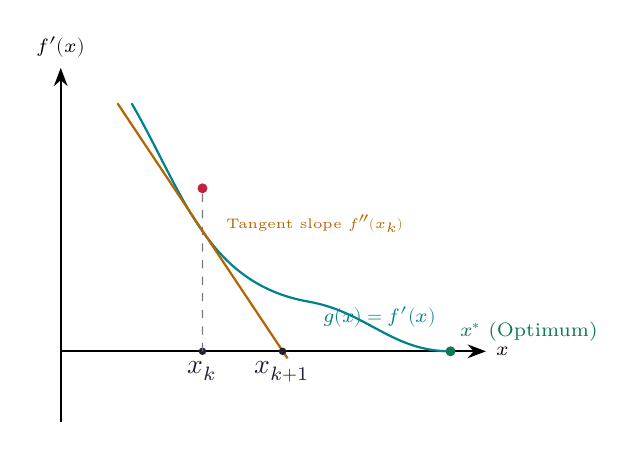
\begin{tikzpicture}[scale=0.9]
  % Draw axes
  \draw[-Stealth, thick] (0,0) -- (6,0) node[right, font=\scriptsize\bfseries] {$x$};
  \draw[-Stealth, thick] (0,-1) -- (0,4) node[above, font=\scriptsize\bfseries] {$f'(x)$};
  
  % Draw curve f'(x)
  \draw[thick, color=myteal] (1,3.5) to[out=-60, in=170] (3.5,0.7) to[out=-10, in=180] (5.5,0);
  \node[above, font=\scriptsize\color{myteal}] at (4.5,0.2) {$g(x) = f'(x)$};

  % Tangent at x_k
  \coordinate (xk) at (2.0,2.3);
  \fill[mydark] (2.0,0) circle (1.5pt) node[below] {$x_k$};
  \fill[myred] (xk) circle (2pt);
  \draw[dashed, color=mydark!60] (2.0,0) -- (xk);
  
  % Tangent line: y - 2.3 = m*(x - 2) -> hits zero at x_k+1
  \draw[thick, color=myamber] (0.8,3.5) -- (3.2,-0.1);
  \node[right, font=\tiny, color=myamber] at (2.2,1.8) {Tangent slope $f''(x_k)$};
  
  % Projections
  \coordinate (xkp1) at (3.13,0);
  \fill[mydark] (xkp1) circle (1.5pt) node[below] {$x_{k+1}$};
  \fill[mygreen] (5.5,0) circle (2pt) node[above right, font=\scriptsize] {$x^*$ (Optimum)};
\end{tikzpicture}
\end{tcolorbox}

% ===============================================================================
\section{Bisection Method}
% ===============================================================================

The bisection method is a robust first-order bracketing technique that solves $f'(x) = 0$ by halving intervals based on sign changes.

\begin{tcolorbox}[defbox, title={Bisection Criterion}]
Let the initial interval be $[a, b]$. If $f'(x)$ is continuous and:
\begin{equation}
  f'(a) \cdot f'(b) < 0
\end{equation}
then by the Intermediate Value Theorem, at least one stationary point $x^*$ exists in $[a, b]$ where $f'(x^*) = 0$.
\end{tcolorbox}

\subsubsection{Algorithm Steps}
\begin{enumerate}[label=\textbf{\arabic*.}, leftmargin=*, itemsep=2.5pt]
  \item Calculate the midpoint: $x_0 = \frac{a+b}{2}$ and evaluate $f'(x_0)$.
  \item If $|f'(x_0)| \le \epsilon$ (tolerance), stop; $x^* \approx x_0$.
  \item If $f'(a) \cdot f'(x_0) < 0$, the root lies in $[a, x_0]$. Set $b = x_0$.
  \item If $f'(x_0) \cdot f'(b) < 0$, the root lies in $[x_0, b]$. Set $a = x_0$.
  \item Repeat until $|b-a| \le \epsilon$. Convergence is guaranteed, though linear and slow.
\end{enumerate}

% ===============================================================================
\section{Secant Method}
% ===============================================================================

The secant method approximates the second derivative $f''(x)$ in the Newton-Raphson formula using two previous evaluations, avoiding analytical differentiation.

\subsection{Iterative Formula}
The curvature is approximated using finite differences between $x_k$ and $x_{k-1}$:
\begin{equation}
  f''(x_k) \approx \frac{f'(x_k) - f'(x_{k-1})}{x_k - x_{k-1}}
\end{equation}
Substituting this into the Newton equation yields the \textbf{Secant Iterative Update}:

\begin{tcolorbox}[formulabox, title={Secant Method Equation}]
\begin{equation}
  x_{k+1} = x_k - f'(x_k) \left[ \frac{x_k - x_{k-1}}{f'(x_k) - f'(x_{k-1})} \right]
\end{equation}
This method requires two initial guess points $x_0$ and $x_1$, and converges superlinearly with a convergence rate of:
\begin{equation}
  \text{Rate } \approx 1.618
\end{equation}
\end{tcolorbox}

% ===============================================================================
\section{Computer Programs / Pseudo-Codes}
% ===============================================================================

\begin{tcolorbox}[tikzbox, title={Newton-Raphson Optimization Pseudo-code}]
\begin{spacing}{1.1}
\begin{verbatim}
Input: Initial guess x0, tolerance eps, max_iter
Output: Local minimum coordinate x*

Function NewtonRaphson(x0, eps, max_iter):
    x = x0
    For k = 1 to max_iter:
        df = FirstDerivative(x)
        ddf = SecondDerivative(x)
        If |ddf| < 1e-12: 
            Print "Error: Curvature close to zero!"
            Return null
        x_new = x - df / ddf
        If |x_new - x| < eps or |df| < eps:
            Return x_new
        x = x_new
    Return x
\end{verbatim}
\end{spacing}
\end{tcolorbox}

\begin{tcolorbox}[tikzbox, title={Secant Optimization Pseudo-code}]
\begin{spacing}{1.1}
\begin{verbatim}
Input: Two initial guesses x0, x1, tolerance eps, max_iter
Output: Local minimum coordinate x*

Function SecantMethod(x0, x1, eps, max_iter):
    x_prev = x0
    x_curr = x1
    For k = 1 to max_iter:
        df_prev = FirstDerivative(x_prev)
        df_curr = FirstDerivative(x_curr)
        If |df_curr - df_prev| < 1e-12:
            Print "Error: Denominator is zero!"
            Return null
        x_next = x_curr - df_curr * (x_curr - x_prev) / (df_curr - df_prev)
        If |x_next - x_curr| < eps:
            Return x_next
        x_prev = x_curr
        x_curr = x_next
    Return x_curr
\end{verbatim}
\end{spacing}
\end{tcolorbox}

\newpage

% ===============================================================================
% MANDATORY QUICK REVISION PAGE
% ===============================================================================
\begin{center}
  {\large\bfseries\color{myred} Quick Revision --- Module 3}\\[3pt]
  {\small\color{mydark} Gradient-Based Methods $|$ OE-EC704B}
\end{center}
\noindent{\color{myred}\rule{\linewidth}{1.2pt}}
\vspace{4pt}

\begin{tcolorbox}[formulabox, title={\textbf{Key Formulas \& Convergence Rates}}]
\renewcommand{\arraystretch}{1.45}
\begin{tabularx}{\linewidth}{B{5.0cm} X}
Newton-Raphson Formula & $x_{k+1} = x_k - \frac{f'(x_k)}{f''(x_k)}$. \\[4pt]
Newton Convergence & Quadratic rate: $e_{k+1} \approx C e_k^2$. \\[4pt]
Bisection Condition & $f'(a) \cdot f'(b) < 0$ \quad (signs must be opposite). \\[4pt]
Secant Update Formula & $x_{k+1} = x_k - f'(x_k) \left[ \frac{x_k - x_{k-1}}{f'(x_k) - f'(x_{k-1})} \right]$. \\[4pt]
Secant Convergence & Superlinear rate: $e_{k+1} \approx C e_k^{1.618}$. \\
\end{tabularx}
\end{tcolorbox}

\begin{tcolorbox}[defbox, title={\textbf{One-Line Definitions}}]
\begin{itemize}[leftmargin=*, itemsep=2.5pt, topsep=0pt]
  \item \textbf{Gradient-Based Optimization:} Minimizing/maximizing functions using directional slope (derivatives) rather than search comparisons alone.
  \item \textbf{Newton-Raphson Method:} An iterative root-finding technique using tangent lines to estimate the point where the derivative is zero.
  \item \textbf{Bisection Method:} A root-finding algorithm that repeatedly bisects an interval and selects a sub-interval in which a sign change occurs.
  \item \textbf{Secant Method:} A gradient-based optimization method that replaces analytical second derivatives with finite difference slope approximations.
  \item \textbf{Quadratic Convergence:} A convergence behavior where the number of correct decimal places roughly doubles with each iteration.
  \item \textbf{Intermediate Value Theorem:} Theorem stating that if a continuous function has opposite signs at interval boundaries, it must cross zero inside.
\end{itemize}
\end{tcolorbox}

\begin{tcolorbox}[exambox, title={\textbf{Frequently Asked / Viva Questions}}]
\begin{enumerate}[topsep=0pt, label=\textbf{Q\arabic*.}, itemsep=5pt]
  \item \Q{Compare Newton-Raphson and Secant methods based on derivative requirements.}
    Newton-Raphson requires evaluating both the first derivative $f'(x)$ and the analytical second derivative $f''(x)$ at each step. The Secant method only requires the first derivative $f'(x)$ because it approximates $f''(x)$ using finite differences.
  \item \Q{State the convergence rate of the Newton-Raphson method and define what it means.}
    It converges quadratically ($e_{k+1} \propto e_k^2$). This means the error in step $k+1$ is proportional to the square of the error in step $k$, leading to extremely rapid convergence near the root.
  \item \Q{Why does the Newton-Raphson method fail if $f''(x_k) = 0$?}
    Because the formula involves dividing by the second derivative. If $f''(x_k) = 0$, the tangent to $f'(x)$ becomes parallel to the x-axis, and the projection point $x_{k+1}$ moves to infinity (division by zero error).
  \item \Q{Explain the role of the sign check $f'(a) \cdot f'(b) < 0$ in the Bisection method.}
    It guarantees that the first derivative $f'(x)$ changes sign across the interval $[a, b]$. For a continuous derivative, this ensures that at least one stationary point (root of $f'(x)=0$) lies within the interval.
  \item \Q{What are the primary disadvantages of the Bisection method?}
    It has a slow, linear convergence rate. It does not utilize the magnitude of the derivative, only its sign, making it take many iterations compared to Newton's method.
  \item \Q{Write down the Secant method update equation.}
    $x_{k+1} = x_k - f'(x_k) \left[ \frac{x_k - x_{k-1}}{f'(x_k) - f'(x_{k-1})} \right]$.
  \item \Q{How does the Secant method differ from the regular False Position (Regula Falsi) root-finding method?}
    False Position always brackets the root and retains points of opposite signs. The Secant method simply uses the last two calculated points, meaning it is not guaranteed to bracket the root and can occasionally diverge.
  \item \Q{What is the convergence rate of the Secant method?}
    It converges superlinearly with order $\alpha = \frac{1+\sqrt{5}}{2} \approx 1.618$ (the Golden Ratio).
  \item \Q{Under what conditions can the Newton-Raphson method diverge?}
    It can diverge if the initial guess $x_0$ is chosen far from the optimum, especially in regions with inflection points, local extrema of $f'(x)$, or flat regions where $f''(x) \approx 0$.
  \item \Q{Write a short MATLAB/Python routine snippet for updating the Secant point.}
    \verb|x_next = x_curr - df_curr * (x_curr - x_prev) / (df_curr - df_prev)| where \verb|df| is the derivative function.
\end{enumerate}
\end{tcolorbox}


% -- Module 4 -----------------------------------------------------------------
\modulestart{4}{Optimality Criteria for Multivariable Functions}

\section{Optimality Criteria for Multivariable Functions}
% ===============================================================================

Let $f(\mathbf{x})$ be a continuous multivariable function defined on the design vector $\mathbf{x} = [x_1, x_2, \dots, x_n]^T$.

\subsection{Necessary Condition (First-Order)}
\begin{tcolorbox}[defbox, title={Theorem: Multivariable Necessary Condition}]
If $f(\mathbf{x})$ is differentiable, a necessary condition for a point $\mathbf{x}^*$ to be a local extremum (minimum or maximum) is that the gradient vector evaluated at $\mathbf{x}^*$ must vanish:
\begin{equation}
  \nabla f(\mathbf{x}^*) = \mathbf{0} \implies \left[ \frac{\partial f}{\partial x_1}, \frac{\partial f}{\partial x_2}, \dots, \frac{\partial f}{\partial x_n} \right]^T_{\mathbf{x} = \mathbf{x}^*} = \mathbf{0}
\end{equation}
Points satisfying this are called \textbf{Stationary Points}.
\end{tcolorbox}

\subsection{Sufficient Condition (Second-Order)}
Optimality is determined by evaluating the \textbf{Hessian Matrix} $H(\mathbf{x}^*)$, defined as the matrix of second-order partial derivatives:
\begin{equation}
  H(\mathbf{x}^*) = \left[ \frac{\partial^2 f}{\partial x_i \partial x_j} \right]_{n \times n}
\end{equation}

\begin{tcolorbox}[defbox, title={Theorem: Multivariable Sufficient Condition}]
At the stationary point $\mathbf{x}^*$:
\begin{itemize}[leftmargin=*, itemsep=2.5pt, topsep=0pt]
  \item If $H(\mathbf{x}^*)$ is \textbf{Positive Definite} (all eigenvalues $> 0$), then $\mathbf{x}^*$ is a \textbf{local minimum}.
  \item If $H(\mathbf{x}^*)$ is \textbf{Negative Definite} (all eigenvalues $< 0$), then $\mathbf{x}^*$ is a \textbf{local maximum}.
  \item If some eigenvalues are positive and others negative, $\mathbf{x}^*$ is a \textbf{Saddle Point}.
\end{itemize}
\end{tcolorbox}

% ===============================================================================
\section{Direct Search Methods (No Gradients)}
% ===============================================================================

Direct search methods do not compute derivatives, making them suitable for noisy or discontinuous functions.

\subsection{Simplex Search Method (Nelder-Mead)}
A simplex in $n$-dimensional space is a geometric figure defined by $n+1$ vertices (e.g., a triangle in 2D, a tetrahedron in 3D). The method moves the simplex toward the optimum using reflection, expansion, contraction, and shrinkage operations.

\begin{tcolorbox}[tikzbox, title={Nelder-Mead Simplex Operations in 2D}]
\centering
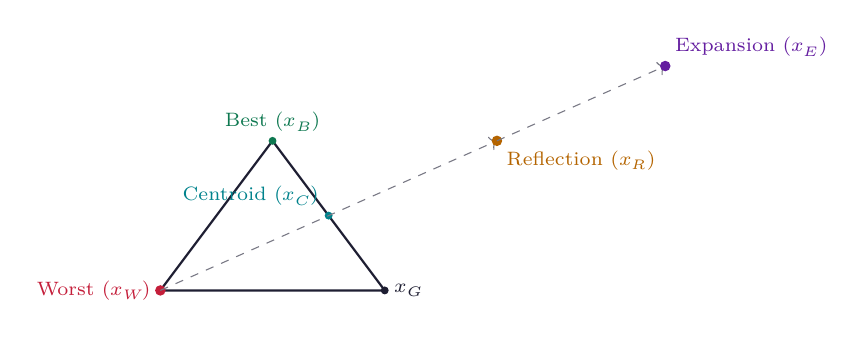
\begin{tikzpicture}[scale=0.95]
  % Define Vertices
  \coordinate (W) at (0,0); % Worst
  \coordinate (G) at (3,0); % Good
  \coordinate (B) at (1.5,2); % Best
  
  % Centroid of G and B
  \coordinate (C) at (2.25,1);
  
  % Simplex triangle
  \draw[thick, color=mydark] (W) -- (G) -- (B) -- cycle;
  \fill[myred] (W) circle (2pt) node[left, font=\scriptsize] {Worst ($x_W$)};
  \fill[mydark] (G) circle (1.5pt) node[right, font=\scriptsize] {$x_G$};
  \fill[mygreen] (B) circle (1.5pt) node[above, font=\scriptsize] {Best ($x_B$)};
  \fill[myteal] (C) circle (1.5pt) node[above left, font=\scriptsize] {Centroid ($x_C$)};
  
  % Operations
  % Reflection: x_R = x_C + (x_C - x_W)
  \coordinate (R) at (4.5,2);
  \draw[dashed, ->, color=mydark!60] (W) -- (R);
  \fill[myamber] (R) circle (2pt) node[below right, font=\scriptsize] {Reflection ($x_R$)};
  
  % Expansion: x_E = x_C + 2(x_C - x_W)
  \coordinate (E) at (6.75,3);
  \draw[dashed, ->, color=mydark!60] (R) -- (E);
  \fill[mypurple] (E) circle (2pt) node[above right, font=\scriptsize] {Expansion ($x_E$)};
\end{tikzpicture}
\end{tcolorbox}

\subsection{Hooke-Jeeves Pattern Search Method}
Hooke-Jeeves is a conceptual search method consisting of two primary components:
\begin{enumerate}[label=\textbf{\arabic*.}, leftmargin=*, itemsep=2.5pt]
  \item \textbf{Exploratory Move:} Performs local searches along the coordinate axes to find a direction of descent.
  \item \textbf{Pattern Move:} Performs an accelerated step along the direction established by connecting successive base points, bypassing slow orthogonal paths.
\end{enumerate}

% ===============================================================================
\section{Gradient-Based Descent Methods}
% ===============================================================================

\subsection{Cauchy's (Steepest Descent) Method}
Steepest descent moves in the direction of the local negative gradient vector, which represents the direction of maximum rate of decrease of the function.

\begin{tcolorbox}[formulabox, title={Steepest Descent Formulation}]
The iterative update equation is:
\begin{equation}
  \mathbf{x}_{k+1} = \mathbf{x}_k - \alpha_k \nabla f(\mathbf{x}_k)
\end{equation}
Where:
\begin{itemize}[leftmargin=*, itemsep=2pt, topsep=0pt]
  \item $\nabla f(\mathbf{x}_k)$ is the gradient vector at step $k$.
  \item $\alpha_k$ is the step length, determined by solving a unidirectional line search problem:
    \begin{equation}
      \text{Minimize } f(\mathbf{x}_k - \alpha \nabla f(\mathbf{x}_k)) \quad \text{w.r.t. } \alpha
    \end{equation}
\end{itemize}
*Characteristics:* Simple to implement but exhibits slow convergence near the optimum due to orthogonal zig-zagging trajectories.
\end{tcolorbox}

\subsection{Newton's Multivariable Method}
Newton's method uses a second-order quadratic approximation of the objective function.

\begin{tcolorbox}[formulabox, title={Newton's Multivariable Update}]
\begin{equation}
  \mathbf{x}_{k+1} = \mathbf{x}_k - [H(\mathbf{x}_k)]^{-1} \nabla f(\mathbf{x}_k)
\end{equation}
Where $[H(\mathbf{x}_k)]^{-1}$ is the inverse of the Hessian matrix.
\par\vspace{3pt}
*Characteristics:* Converges quadratically (extremely fast near the optimum) but requires calculating and inverting the Hessian matrix at every step, which is computationally expensive for large systems.
\end{tcolorbox}

% ===============================================================================
\section{Multi-Objective and Pareto Optimization}
% ===============================================================================

In real-world engineering, we often optimize multiple conflicting objectives simultaneously (e.g., minimizing cost while maximizing safety).

\subsection{Pareto Dominance \& Optimality}
Instead of a single optimum, multi-objective optimization yields a set of trade-off solutions.

\begin{tcolorbox}[defbox, title={Definition of Pareto Dominance}]
A decision vector $\mathbf{x}_1$ is said to \textbf{dominate} $\mathbf{x}_2$ if:
\begin{enumerate}[label=\textbf{\arabic*.}, leftmargin=*, itemsep=2pt, topsep=0pt]
  \item $\mathbf{x}_1$ is no worse than $\mathbf{x}_2$ in all objectives.
  \item $\mathbf{x}_1$ is strictly better than $\mathbf{x}_2$ in at least one objective.
\end{enumerate}
A solution is \textbf{Pareto Optimal} if it is not dominated by any other feasible solution. The set of all Pareto optimal solutions in the objective space forms the \textbf{Pareto Front}.
\end{tcolorbox}

\begin{tcolorbox}[tikzbox, title={Pareto Optimal Front (Conflicting Objectives)}]
\centering
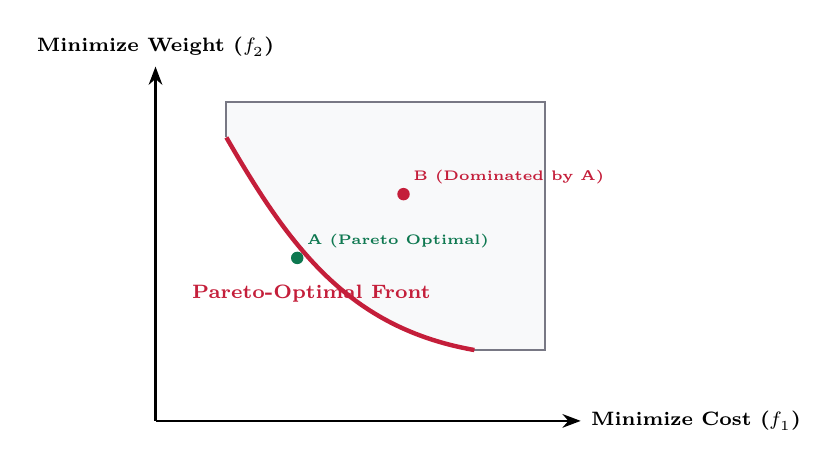
\begin{tikzpicture}[scale=0.9]
  \draw[-Stealth, thick] (0,0) -- (6,0) node[right, font=\scriptsize\bfseries] {Minimize Cost ($f_1$)};
  \draw[-Stealth, thick] (0,0) -- (0,5) node[above, font=\scriptsize\bfseries] {Minimize Weight ($f_2$)};
  
  % Feasible Region Shading
  \fill[mygray, opacity=0.8] (1,4) to[out=-60, in=170] (4.5,1) -- (5.5,1) -- (5.5,4.5) -- (1,4.5) -- cycle;
  \draw[thick, color=mydark!60] (1,4) -- (1,4.5) -- (5.5,4.5) -- (5.5,1) -- (4.5,1);
  
  % Pareto Curve
  \draw[ultra thick, color=myred] (1,4) to[out=-60, in=170] (4.5,1);
  \node[color=myred, font=\scriptsize\bfseries] at (2.2,1.8) {Pareto-Optimal Front};
  
  % Solution points
  \fill[mygreen] (2,2.3) circle (2.5pt) node[above right, font=\tiny\bfseries] {A (Pareto Optimal)};
  \fill[myred] (3.5,3.2) circle (2.5pt) node[above right, font=\tiny\bfseries] {B (Dominated by A)};
\end{tikzpicture}
\end{tcolorbox}

\newpage

% ===============================================================================
% MANDATORY QUICK REVISION PAGE
% ===============================================================================
\begin{center}
  {\large\bfseries\color{myred} Quick Revision --- Module 4}\\[3pt]
  {\small\color{mydark} Multivariable Optimization $|$ OE-EC704B}
\end{center}
\noindent{\color{myred}\rule{\linewidth}{1.2pt}}
\vspace{4pt}

\begin{tcolorbox}[formulabox, title={\textbf{Key Concepts \& Mathematical Rules}}]
\renewcommand{\arraystretch}{1.45}
\begin{tabularx}{\linewidth}{B{5.0cm} X}
Gradient Vector ($\nabla f$) & $\nabla f = \left[ \frac{\partial f}{\partial x_1}, \frac{\partial f}{\partial x_2}, \dots, \frac{\partial f}{\partial x_n} \right]^T = \mathbf{0}$. \\[4pt]
Hessian Matrix ($H$) & $H_{ij} = \frac{\partial^2 f}{\partial x_i \partial x_j}$ \quad (square symmetric matrix). \\[4pt]
Cauchy's Update & $\mathbf{x}_{k+1} = \mathbf{x}_k - \alpha_k \nabla f(\mathbf{x}_k)$ \quad (Steepest Descent). \\[4pt]
Newton's Update & $\mathbf{x}_{k+1} = \mathbf{x}_k - H^{-1} \nabla f(\mathbf{x}_k)$ \quad (Quadratic Convergence). \\[4pt]
Pareto Dominance Rule & $\mathbf{x}_1 \prec \mathbf{x}_2 \iff \forall i: f_i(\mathbf{x}_1) \le f_i(\mathbf{x}_2)$ and $\exists j: f_j(\mathbf{x}_1) < f_j(\mathbf{x}_2)$. \\
\end{tabularx}
\end{tcolorbox}

\begin{tcolorbox}[defbox, title={\textbf{One-Line Definitions}}]
\begin{itemize}[leftmargin=*, itemsep=2.5pt, topsep=0pt]
  \item \textbf{Positive Definite Matrix:} A matrix whose eigenvalues are all strictly positive (indicates local minimum structure).
  \item \textbf{Saddle Point:} A stationary point at which the Hessian matrix is indefinite (eigenvalues of mixed signs).
  \item \textbf{Nelder-Mead Simplex:} A derivative-free search method using vertices of a geometric figure to crawl toward the optimum.
  \item \textbf{Hooke-Jeeves Method:} A coordinate-based search method combining local exploratory moves and pattern acceleration.
  \item \textbf{Steepest Descent:} An iterative gradient method moving in the direction of the local negative gradient vector.
  \item \textbf{Pareto Front:} The set of all non-dominated solutions representing optimal trade-offs in multi-objective problems.
\end{itemize}
\end{tcolorbox}

\begin{tcolorbox}[exambox, title={\textbf{Frequently Asked / Viva Questions}}]
\begin{enumerate}[topsep=0pt, label=\textbf{Q\arabic*.}, itemsep=5pt]
  \item \Q{State the necessary and sufficient conditions for a local minimum of a multivariable function.}
    Necessary condition: The gradient vector must vanish, $\nabla f(\mathbf{x}^*) = \mathbf{0}$. Sufficient condition: The Hessian matrix $H(\mathbf{x}^*)$ must be positive definite.
  \item \Q{What is a Hessian matrix and what is its role in multivariable optimization?}
    The Hessian is a square symmetric matrix of second-order partial derivatives. Its role is to provide local curvature information to identify if a stationary point is a minimum, maximum, or saddle point.
  \item \Q{Explain why Cauchy's (Steepest Descent) method exhibits a zig-zag search trajectory.}
    Because successive search directions in Cauchy's method are mathematically orthogonal: $\mathbf{d}_k \cdot \mathbf{d}_{k-1} = 0$. This perpendicular stepping causes the algorithm to bounce back and forth in narrow valleys.
  \item \Q{What are the operations performed in the Nelder-Mead simplex search method?}
    The operations are Reflection, Expansion, Contraction (Outer and Inner), and Shrinkage.
  \item \Q{Differentiate between exploratory and pattern moves in the Hooke-Jeeves method.}
    An exploratory move searches along the coordinate axes to find a local descending direction. A pattern move accelerates the search by stepping along the vector connecting successive base points.
  \item \Q{Compare multivariable Newton's method with the Steepest Descent method.}
    Newton's method converges quadratically (very fast) but requires calculating and inverting the Hessian matrix. Steepest descent only requires the first-order gradient, making it computationally simpler per step but much slower to converge.
  \item \Q{What is Pareto optimality in multi-objective optimization?}
    A solution is Pareto optimal if no other solution exists that improves one objective without simultaneously degrading at least one other objective.
  \item \Q{Define the concept of a saddle point.}
    A saddle point is a stationary point where the gradient is zero, but the Hessian is indefinite, meaning the function increases in some directions and decreases in others.
  \item \Q{What is the purpose of a unidirectional line search in multivariable algorithms?}
    To find the optimal step length $\alpha_k$ that minimizes the function along the selected search direction $\mathbf{d}_k$: $\min_\alpha f(\mathbf{x}_k + \alpha \mathbf{d}_k)$.
  \item \Q{What makes a matrix positive definite using Sylvester's Criterion?}
    A symmetric matrix is positive definite if and only if all its leading principal minors (determinants of top-left submatrices) are strictly positive.
\end{enumerate}
\end{tcolorbox}


% -- Module 5 -----------------------------------------------------------------
\modulestart{5}{Characteristics of Constrained Problems}

\section{Characteristics of Constrained Problems}
% ===============================================================================

Constrained optimization restricts the search space to a feasible region. Let us analyze the constraint boundaries:

\begin{tcolorbox}[defbox, title={Active vs. Inactive Constraints}]
At a candidate design point $\mathbf{x}$:
\begin{itemize}[leftmargin=*, itemsep=2.5pt, topsep=0pt]
  \item An inequality constraint $g_j(\mathbf{x}) \le 0$ is said to be \textbf{Active} if $g_j(\mathbf{x}) = 0$. The point lies exactly on the boundary of that constraint.
  \item It is \textbf{Inactive} if $g_j(\mathbf{x}) < 0$. The constraint is satisfied, and the point lies in the interior of the feasible space.
  \item It is \textbf{Violated} if $g_j(\mathbf{x}) > 0$. The design point is infeasible.
\end{itemize}
All equality constraints $h_k(\mathbf{x}) = 0$ must be active at all feasible points.
\end{tcolorbox}

\begin{tcolorbox}[tikzbox, title={Feasible Region and Constrained Optimum}]
\centering
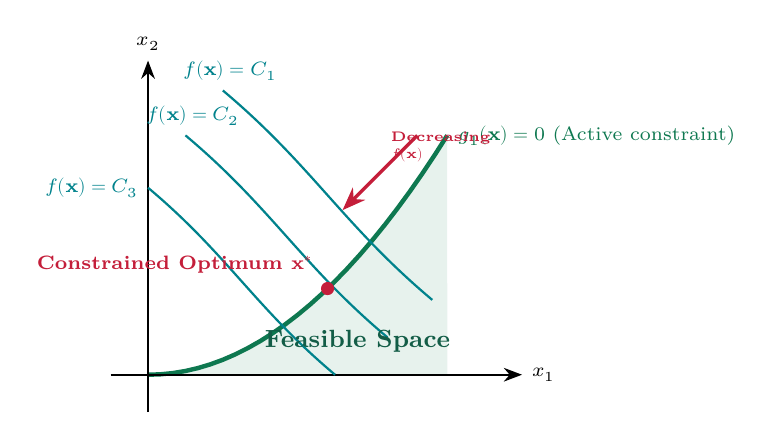
\begin{tikzpicture}[scale=0.95]
  % Feasible area shading
  \fill[mygreen!10] (0,0) plot[domain=0:4] (\x, {0.2*\x*\x}) -- (4,0) -- cycle;
  \draw[ultra thick, color=mygreen] (0,0) plot[domain=0:4] (\x, {0.2*\x*\x}) node[right, font=\scriptsize] {$g_1(\mathbf{x}) = 0$ (Active constraint)};
  
  % Axes
  \draw[-Stealth, thick] (-0.5,0) -- (5,0) node[right, font=\scriptsize\bfseries] {$x_1$};
  \draw[-Stealth, thick] (0,-0.5) -- (0,4.2) node[above, font=\scriptsize\bfseries] {$x_2$};
  
  % Contours of f(x)
  \draw[thick, color=myteal] (1.0, 3.8) to[out=-40, in=140] (3.8, 1.0);
  \node[above, font=\scriptsize, color=myteal] at (1.1,3.8) {$f(\mathbf{x}) = C_1$};
  
  \draw[thick, color=myteal] (0.5, 3.2) to[out=-40, in=140] (3.2, 0.5);
  \node[above, font=\scriptsize, color=myteal] at (0.6,3.2) {$f(\mathbf{x}) = C_2$};
  
  \draw[thick, color=myteal] (0.0, 2.5) to[out=-40, in=140] (2.5, 0.0);
  \node[left, font=\scriptsize, color=myteal] at (0.0,2.5) {$f(\mathbf{x}) = C_3$};
  
  % Decreasing Direction Arrow
  \draw[-Stealth, very thick, color=myred] (3.6, 3.2) -- (2.6, 2.2) 
    node[midway, above right, font=\tiny\bfseries\color{myred}, align=left] {Decreasing\\$f(\mathbf{x})$};

  % Feasible text
  \node[color=mygreen!70!mydark, font=\small\bfseries] at (2.8, 0.45) {Feasible Space};
  
  % Optimum Point
  \coordinate (opt) at (2.4, 1.152);
  \fill[myred] (opt) circle (2.5pt);
  \node[above left, font=\scriptsize\bfseries, color=myred, xshift=-2pt, yshift=2pt] at (opt) {Constrained Optimum $\mathbf{x}^*$};
\end{tikzpicture}
\end{tcolorbox}

% ===============================================================================
\section{Direct Constrained Optimization Methods}
% ===============================================================================

Direct methods evaluate only function values and directly handle constraints by adjusting candidate coordinates.

\subsection{Box's Complex Method}
Box's Complex Method is an extension of the Nelder-Mead Simplex method designed to handle inequality constraints:
\begin{itemize}[leftmargin=*, itemsep=2.5pt]
  \item Uses a geometric shape called a \textbf{Complex} consisting of $k \ge n+1$ vertices (typically $k = 2n$).
  \item If a generated reflection point violates an inequality constraint, it is moved halfway toward the centroid of the remaining feasible points until it becomes feasible.
\end{itemize}

\subsection{Kelly's Cutting Plane Method}
Kelly's Cutting Plane Method solves non-linear convex constrained problems:
\begin{enumerate}[label=\textbf{\arabic*.}, leftmargin=*, itemsep=2.5pt]
  \item Linearizes all non-linear constraints using first-order Taylor expansions to form a linear programming (LP) relaxation.
  \item Solves the LP relaxation. If the solution is infeasible for the original non-linear constraints, it adds a new linear inequality constraint (a \textbf{Cutting Plane}) that slices off the infeasible LP solution.
  \item Repeats the process until convergence, generating a sequence of tightening linear hulls.
\end{enumerate}

% ===============================================================================
\section{Indirect Methods (Transformation Techniques)}
% ===============================================================================

Transformation techniques reformulate a constrained problem into an equivalent sequence of unconstrained problems.

\subsection{Exterior Penalty Function Method}
The exterior penalty method starts search in the infeasible region and penalizes constraint violations, forcing iterations toward the feasible boundary.

\begin{tcolorbox}[formulabox, title={Exterior Penalty Function Formulation}]
The unconstrained penalty objective function $\Phi$ is defined as:
\begin{equation}
  \Phi(\mathbf{x}, r_p) = f(\mathbf{x}) + r_p \sum_{j=1}^m \left[ \max\left(0, g_j(\mathbf{x})\right) \right]^2 + \frac{1}{r_p} \sum_{k=1}^p \left[ h_k(\mathbf{x}) \right]^2
\end{equation}
Where $r_p$ is a positive penalty parameter.
\par\vspace{3pt}
*Algorithm:*
\begin{enumerate}[label=\textbf{\arabic*.}, leftmargin=*, itemsep=2.5pt]
  \item Select an initial penalty value $r_p^{(1)}$ (usually small) and minimize $\Phi(\mathbf{x}, r_p^{(1)})$ unconstrained.
  \item Increase the parameter: $r_p^{(k+1)} = c \cdot r_p^{(k)}$ (where $c > 1$).
  \item Re-minimize $\Phi$. As $r_p \to \infty$, the sequence of unconstrained minima converges to the constrained optimum $\mathbf{x}^*$.
\end{enumerate}
\end{tcolorbox}

\subsection{Interior Penalty (Barrier) Function Method}
The interior penalty method starts inside the feasible region and creates a barrier at the boundary that prevents iterations from escaping into the infeasible space.

\begin{tcolorbox}[formulabox, title={Interior Barrier Function Formulations}]
The unconstrained barrier objective function $\Phi$ is defined using one of two barriers:
\begin{itemize}[leftmargin=*, itemsep=3pt, topsep=0pt]
  \item \textbf{Inverse Barrier Function:}
    \begin{equation}
      \Phi(\mathbf{x}, r_k) = f(\mathbf{x}) - r_k \sum_{j=1}^m \frac{1}{g_j(\mathbf{x})}
    \end{equation}
  \item \textbf{Logarithmic Barrier Function:}
    \begin{equation}
      \Phi(\mathbf{x}, r_k) = f(\mathbf{x}) - r_k \sum_{j=1}^m \ln\left[ -g_j(\mathbf{x}) \right]
    \end{equation}
\end{itemize}
Where $r_k$ is the positive barrier parameter.
\par\vspace{3pt}
*Algorithm:*
\begin{enumerate}[label=\textbf{\arabic*.}, leftmargin=*, itemsep=2.5pt]
  \item Start at a strictly feasible point. Minimize $\Phi(\mathbf{x}, r_k^{(1)})$.
  \item Decrease the parameter: $r_k^{(k+1)} = d \cdot r_k^{(k)}$ (where $0 < d < 1$).
  \item Re-minimize. As $r_k \to 0$, the barrier effect weakens at the boundary, allowing convergence to the boundary optimum $\mathbf{x}^*$.
\end{enumerate}
\end{tcolorbox}

% ===============================================================================
\section{Convex Optimization Methods}
% ===============================================================================

Convex optimization is a special class of optimization with unique mathematical guarantees.

\begin{tcolorbox}[defbox, title={Convex Programming Problem}]
A constrained optimization problem is a \textbf{Convex Programming Problem} if:
\begin{enumerate}[label=\textbf{\arabic*.}, leftmargin=*, itemsep=2pt, topsep=0pt]
  \item The objective function $f(\mathbf{x})$ is convex.
  \item All inequality constraints $g_j(\mathbf{x}) \le 0$ are convex functions.
  \item All equality constraints $h_k(\mathbf{x}) = 0$ are linear (affine) functions.
\end{enumerate}
\end{tcolorbox}

\textbf{Theorem:} For a convex programming problem, \textbf{any local minimum is guaranteed to be the global minimum}, eliminating the risk of getting trapped in local sub-optimal states.

\newpage

% ===============================================================================
% MANDATORY QUICK REVISION PAGE
% ===============================================================================
\begin{center}
  {\large\bfseries\color{myred} Quick Revision --- Module 5}\\[3pt]
  {\small\color{mydark} Constrained Optimization $|$ OE-EC704B}
\end{center}
\noindent{\color{myred}\rule{\linewidth}{1.2pt}}
\vspace{4pt}

\begin{tcolorbox}[formulabox, title={\textbf{Key Concepts \& Formulations}}]
\renewcommand{\arraystretch}{1.45}
\begin{tabularx}{\linewidth}{B{5.0cm} X}
Active Inequality & $g_j(\mathbf{x}^*) = 0$ \quad (optimum lies on the constraint boundary). \\[4pt]
Inactive Inequality & $g_j(\mathbf{x}^*) < 0$ \quad (constraint is satisfied with slack). \\[4pt]
Exterior Penalty $\Phi$ & $\Phi = f(\mathbf{x}) + r_p \sum [\max(0, g_j)]^2$ \quad (where $r_p \to \infty$). \\[4pt]
Inverse Interior Barrier & $\Phi = f(\mathbf{x}) - r_k \sum \frac{1}{g_j}$ \quad (where $r_k \to 0$). \\[4pt]
Logarithmic Barrier & $\Phi = f(\mathbf{x}) - r_k \sum \ln(-g_j)$ \quad (where $r_k \to 0$). \\[4pt]
Convex Definition & $f(\lambda \mathbf{x} + (1-\lambda)\mathbf{y}) \le \lambda f(\mathbf{x}) + (1-\lambda)f(\mathbf{y})$ for $\lambda \in [0, 1]$. \\
\end{tabularx}
\end{tcolorbox}

\begin{tcolorbox}[defbox, title={\textbf{One-Line Definitions}}]
\begin{itemize}[leftmargin=*, itemsep=2.5pt, topsep=0pt]
  \item \textbf{Active Constraint:} A constraint whose boundary passes directly through the current design point.
  \item \textbf{Complex Method:} A constrained direct search method utilizing $2n$ vertices to explore bounded spaces.
  \item \textbf{Transformation Technique:} Reformulating constrained problems into sequential unconstrained formulations.
  \item \textbf{Exterior Penalty Method:} A transformation technique that approaches the boundary from the infeasible design region.
  \item \textbf{Interior Barrier Method:} A transformation technique that approaches the boundary from strictly within the feasible region.
  \item \textbf{Convex Function:} A function where a line segment connecting any two points on its graph lies above or on the graph.
\end{itemize}
\end{tcolorbox}

\begin{tcolorbox}[exambox, title={\textbf{Frequently Asked / Viva Questions}}]
\begin{enumerate}[topsep=0pt, label=\textbf{Q\arabic*.}, itemsep=5pt]
  \item \Q{What is the difference between active and inactive constraints at an optimum point?}
    An active constraint satisfies $g_j(\mathbf{x}^*) = 0$ (lies on the boundary). An inactive constraint satisfies $g_j(\mathbf{x}^*) < 0$ (lies inside the boundary) and does not limit the local optimum.
  \item \Q{Compare the search paths of the Exterior Penalty and Interior Barrier methods.}
    The exterior penalty method starts from an infeasible point and moves inward toward the feasible boundary as $r_p \to \infty$. The interior barrier method starts from a strictly feasible point and moves outward toward the boundary as $r_k \to 0$.
  \item \Q{Why does the Interior Barrier method require a strictly feasible starting point?}
    Because the barrier terms (such as $1/g_j$ or $\ln(-g_j)$) are mathematically undefined or return complex/imaginary values in the infeasible region ($g_j(\mathbf{x}) > 0$).
  \item \Q{State Sylvester's conditions for a function to be strictly convex.}
    A function is strictly convex if its Hessian matrix $H(\mathbf{x})$ is positive definite (all eigenvalues $> 0$) at all points in the design space.
  \item \Q{What is the main advantage of Convex Programming?}
    Any local minimum of a convex programming problem is guaranteed to be the global minimum.
  \item \Q{Explain the concept behind Kelly's Cutting Plane method.}
    It linearizes the non-linear constraints to solve an approximating linear program. It then iteratively adds linear constraint inequalities (cutting planes) to cut off infeasible areas.
  \item \Q{Why are equality constraints challenging for the Interior Barrier method?}
    Because equality constraints $h_k(\mathbf{x}) = 0$ define a region with zero thickness, leaving no "interior" space to start a strictly feasible search path.
  \item \Q{How does Box's Complex method handle constraint violations?}
    If a generated point is infeasible, it is iteratively retracted halfway toward the centroid of the remaining feasible points until it becomes feasible.
  \item \Q{Write down the logarithmic barrier objective function expression.}
    $\Phi(\mathbf{x}, r_k) = f(\mathbf{x}) - r_k \sum_{j=1}^m \ln(-g_j(\mathbf{x}))$.
  \item \Q{What is the physical meaning of the penalty parameter $r_p$ in the exterior penalty method?}
    It acts as a scaling coefficient for constraint violations. As $r_p \to \infty$, the penalty for violating constraints becomes extremely large, forcing the unconstrained optimizer to find a feasible solution.
\end{enumerate}
\end{tcolorbox}


% -- Module 6 -----------------------------------------------------------------
\modulestart{6}{Genetic Algorithm (GA)}

\section{Genetic Algorithm (GA)}
% ===============================================================================

Genetic Algorithms are global meta-heuristic search algorithms inspired by Charles Darwin's theory of natural evolution (survival of the fittest). They operate on a population of candidate designs represented as chromosomes.

\subsection{Basic Genetic Operators}
A standard GA processes a population using three core operators:
\begin{enumerate}[label=\textbf{\arabic*.}, leftmargin=*, itemsep=3.5pt]
  \item \textbf{Selection (Reproduction):} Identifies and copies high-fitness individuals to a mating pool.
    \begin{itemize}[label=\tiny$\bullet$, leftmargin=1.5em, itemsep=2pt]
      \item \textit{Roulette Wheel Selection:} Probability of selecting individual $i$ is proportional to its fitness $f_i$:
        \begin{equation}
          p_i = \frac{f_i}{\sum_{j=1}^N f_j}
        \end{equation}
      \item \textit{Tournament Selection:} Randomly selects a few individuals and chooses the best.
    \end{itemize}
  \item \textbf{Crossover (Recombination):} Combines genetic material from two parent chromosomes to create offspring.
    \begin{itemize}[label=\tiny$\bullet$, leftmargin=1.5em, itemsep=2pt]
      \item \textit{Single-Point Crossover:} Parents are split at a random point and swapped.
      \item \textit{Multi-Point Crossover:} Multiple split boundaries are defined.
    \end{itemize}
  \item \textbf{Mutation:} Randomly flips bits or values in a chromosome with a small probability ($p_m \approx 0.005$) to maintain diversity and prevent premature convergence.
\end{enumerate}

\subsection{The Genetic Algorithm Flowchart}
The iterative lifecycle of a GA is mapped below:

\begin{tcolorbox}[tikzbox, title={Genetic Algorithm Search Loop}]
\centering
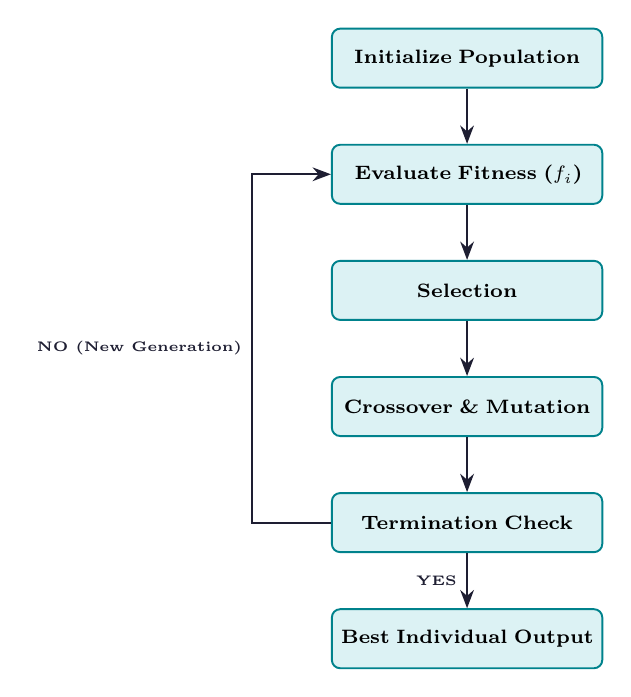
\begin{tikzpicture}[
  node distance=0.7cm and 1.5cm,
  block/.style={rectangle, draw=myteal, fill=hdrteal, text width=3.2cm, align=center, minimum height=0.75cm, font=\scriptsize\bfseries, rounded corners=3pt, line width=0.7pt},
  arrow/.style={-Stealth, thick, color=mydark}
]
  \node[block] (s1) {Initialize Population};
  \node[block, below=of s1] (s2) {Evaluate Fitness ($f_i$)};
  \node[block, below=of s2] (s3) {Selection};
  \node[block, below=of s3] (s4) {Crossover \& Mutation};
  \node[block, below=of s4] (s5) {Termination Check};
  \node[block, below=of s5] (s6) {Best Individual Output};

  \draw[arrow] (s1) -- (s2);
  \draw[arrow] (s2) -- (s3);
  \draw[arrow] (s3) -- (s4);
  \draw[arrow] (s4) -- (s5);
  \draw[arrow] (s5) -- node[left, font=\tiny\bfseries\color{mygreen}] {YES} (s6);
  
  \draw[arrow] (s5.west) -- ++(-1.0,0) |- node[pos=0.25, left, font=\tiny\bfseries\color{myred}] {NO (New Generation)} (s2.west);
\end{tikzpicture}
\end{tcolorbox}

% ===============================================================================
\section{Simulated Annealing (SA)}
% ===============================================================================

Simulated Annealing is inspired by the physical process of annealing in metallurgy, where a metal is heated to a high temperature and cooled slowly to minimize internal energy, forming a perfect crystal lattice.

\subsection{The Metropolis Acceptance Criterion}
SA allows uphill moves (accepting worse designs) to escape local minima. Let the change in objective value be $\Delta E = f(\mathbf{x}_{new}) - f(\mathbf{x}_{old})$.

\begin{tcolorbox}[formulabox, title={Metropolis Criterion Equations}]
\begin{itemize}[leftmargin=*, itemsep=3.5pt, topsep=0pt]
  \item If $\Delta E < 0$ (improvement), the new state is \textbf{always accepted}: $P(Accept) = 1$.
  \item If $\Delta E \ge 0$ (worse state), the new state is accepted with a \textbf{Boltzmann probability}:
    \begin{equation}
      P(Accept) = \exp\left( -\frac{\Delta E}{T} \right)
    \end{equation}
    Where $T$ is the virtual temperature.
\end{itemize}
\par\vspace{3pt}
As the temperature $T$ is slowly reduced using a cooling schedule (e.g., $T_{k+1} = \alpha T_k$ with $0.8 \le \alpha < 1.0$), the probability of accepting worse moves approaches 0, and the algorithm converges to the global minimum.
\end{tcolorbox}

% ===============================================================================
\section{Swarm Intelligence Algorithms}
% ===============================================================================

Swarm intelligence algorithms mimic the collective behavior of decentralized, self-organized biological swarms.

\subsection{Particle Swarm Optimization (PSO)}
PSO is inspired by bird flocking. A swarm of particles moves through the design space, where each particle tracks its own personal best position ($\mathbf{p}_{best, i}$) and the swarm's global best position ($\mathbf{g}_{best}$).

\begin{tcolorbox}[formulabox, title={PSO Particle Update Equations}]
At generation $t+1$, the velocity vector $\mathbf{v}_i$ and position vector $\mathbf{x}_i$ of particle $i$ are updated as:
\begin{equation}
  \mathbf{v}_i^{(t+1)} = w \mathbf{v}_i^{(t)} + c_1 r_1 \left( \mathbf{p}_{best, i} - \mathbf{x}_i^{(t)} \right) + c_2 r_2 \left( \mathbf{g}_{best} - \mathbf{x}_i^{(t)} \right)
\end{equation}
\begin{equation}
  \mathbf{x}_i^{(t+1)} = \mathbf{x}_i^{(t)} + \mathbf{v}_i^{(t+1)}
\end{equation}
Where:
\begin{itemize}[leftmargin=*, itemsep=2.0pt, topsep=0pt]
  \item $w$ is the \textbf{inertia weight} regulating momentum.
  \item $c_1$ (cognitive parameter) and $c_2$ (social parameter) are acceleration constants.
  \item $r_1, r_2$ are random numbers uniformly distributed in $[0, 1]$.
\end{itemize}
\end{tcolorbox}

\subsection{Swarm Variants: DE, BFA, and ACO}
\begin{itemize}[leftmargin=*, itemsep=4pt]
  \item \textbf{Differential Evolution (DE):} A vector-based evolutionary algorithm that creates new candidate vectors by adding weighted differences between random population vectors to a target vector, followed by crossover and selection.
  \item \textbf{Bacterial Foraging Algorithm (BFA):} Mimics the chemotaxis (swimming and tumbling), reproduction, and dispersal behaviors of E. coli bacteria.
  \item \textbf{Ant Colony Optimization (ACO):} Mimics the foraging behavior of real ants, which communicate path lengths using chemical pheromones.
\end{itemize}

\begin{tcolorbox}[formulabox, title={Ant Colony Pheromone Update Rule}]
The pheromone level $\tau_{ij}$ on path segment $(i, j)$ is updated after each iteration as:
\begin{equation}
  \tau_{ij} = (1 - \rho)\tau_{ij} + \sum_{k=1}^m \Delta \tau_{ij}^k
\end{equation}
Where:
\begin{itemize}[leftmargin=*, itemsep=2.0pt, topsep=0pt]
  \item $\rho$ is the \textbf{pheromone evaporation rate} ($0 < \rho \le 1$), preventing infinite accumulation.
  \item $\Delta \tau_{ij}^k$ is the pheromone deposited by ant $k$: $\Delta \tau_{ij}^k = \frac{Q}{L_k}$ if ant $k$ traversed segment $(i, j)$ (where $L_k$ is the total path length, and $Q$ is a constant).
\end{itemize}
\end{tcolorbox}

\newpage

% ===============================================================================
% MANDATORY QUICK REVISION PAGE
% ===============================================================================
\begin{center}
  {\large\bfseries\color{myred} Quick Revision --- Module 6}\\[3pt]
  {\small\color{mydark} Advanced Swarm Algorithms $|$ OE-EC704B}
\end{center}
\noindent{\color{myred}\rule{\linewidth}{1.2pt}}
\vspace{4pt}

\begin{tcolorbox}[formulabox, title={\textbf{Key Concepts \& Swarm Metrics}}]
\renewcommand{\arraystretch}{1.45}
\begin{tabularx}{\linewidth}{B{5.0cm} X}
Selection Probability & $p_i = f_i / \sum f_j$ \quad (Roulette Wheel). \\[4pt]
Boltzmann Probability & $P(Accept) = \exp(-\Delta E / T)$ \quad (Simulated Annealing). \\[4pt]
PSO Velocity Update & $\mathbf{v}_i^{(t+1)} = w \mathbf{v}_i^{(t)} + c_1 r_1 (\mathbf{p}_{best} - \mathbf{x}_i) + c_2 r_2 (\mathbf{g}_{best} - \mathbf{x}_i)$. \\[4pt]
PSO Position Update & $\mathbf{x}_i^{(t+1)} = \mathbf{x}_i^{(t)} + \mathbf{v}_i^{(t+1)}$. \\[4pt]
ACO Pheromone Update & $\tau_{ij} \leftarrow (1-\rho)\tau_{ij} + \sum \Delta \tau_{ij}^k$ \quad ($\rho$ is evaporation rate). \\
\end{tabularx}
\end{tcolorbox}

\begin{tcolorbox}[defbox, title={\textbf{One-Line Definitions}}]
\begin{itemize}[leftmargin=*, itemsep=2.5pt, topsep=0pt]
  \item \textbf{Meta-heuristic Algorithm:} A high-level search heuristic designed to find, generate, or select a search path to solve global optimization problems.
  \item \textbf{Crossover Operator:} A GA operator that recombines parts of two parent chromosomes to produce offspring.
  \item \textbf{Elitism:} A GA technique that copies the best-performing chromosomes directly to the next generation without changes.
  \item \textbf{Annealing Cooling Schedule:} A function detailing how the virtual temperature $T$ is systematically reduced during Simulated Annealing.
  \item \textbf{Inertia Weight ($w$):} A PSO parameter controlling the influence of a particle's historical velocity on its current trajectory.
  \item \textbf{Chemotaxis:} The direct movement of E. coli bacteria along chemical gradients, consisting of alternating swims and tumbles.
\end{itemize}
\end{tcolorbox}

\begin{tcolorbox}[exambox, title={\textbf{Frequently Asked / Viva Questions}}]
\begin{enumerate}[topsep=0pt, label=\textbf{Q\arabic*.}, itemsep=5pt]
  \item \Q{Explain the three primary operators used in standard Genetic Algorithms.}
    The operators are: Selection (copies high-fitness chromosomes to the mating pool), Crossover (recombines genetic sequences from parent pairs to create offspring), and Mutation (randomly alters genes to maintain population diversity).
  \item \Q{How does Roulette Wheel selection work?}
    In Roulette Wheel selection, the selection probability of an individual is proportional to its fitness value. Highly fit individuals occupy a larger slice of the virtual wheel, increasing their chances of being chosen.
  \item \Q{What is simulated annealing and what is its thermodynamic analogy?}
    SA is a global optimization algorithm. Its thermodynamic analogy is the slow cooling (annealing) of a molten metal to achieve a low-energy, highly structured crystal lattice, which corresponds to the global minimum.
  \item \Q{Why does Simulated Annealing accept worse designs, and how does it prevent divergence?}
    It accepts worse designs to climb out of local minima traps. It prevents divergence by reducing the acceptance probability ($e^{-\Delta E/T}$) as the virtual temperature $T$ cools, making the search purely local at the end.
  \item \Q{Write down the velocity update equation for Particle Swarm Optimization (PSO).}
    $\mathbf{v}_i^{(t+1)} = w \mathbf{v}_i^{(t)} + c_1 r_1 \left( \mathbf{p}_{best, i} - \mathbf{x}_i^{(t)} \right) + c_2 r_2 \left( \mathbf{g}_{best} - \mathbf{x}_i^{(t)} \right)$.
  \item \Q{Define the cognitive and social terms in the PSO update equations.}
    The cognitive term ($c_1 r_1(\mathbf{p}_{best} - \mathbf{x})$) pulls the particle toward its own personal historical best. The social term ($c_2 r_2(\mathbf{g}_{best} - \mathbf{x})$) pulls the particle toward the global best found by the entire swarm.
  \item \Q{What is the role of pheromone evaporation in Ant Colony Optimization (ACO)?}
    It systematically decreases the pheromone levels on all paths ($1-\rho$). This prevents the algorithm from getting stuck in early sub-optimal paths by allowing alternative pathways to compete.
  \item \Q{How does the Differential Evolution (DE) algorithm generate new candidate vectors?}
    It creates new trial vectors by adding a weighted difference vector between two random population members to a third vector, followed by crossover and selection.
  \item \Q{List the three operational steps of the Bacterial Foraging Algorithm (BFA).}
    Chemotaxis (swimming and tumbling), Reproduction (splitting healthy bacteria), and Elimination and Dispersal (dispersing bacteria randomly to model environmental shocks).
  \item \Q{What is Elitism in Genetic Algorithms and why is it used?}
    Elitism is the process of copying the absolute best individual(s) directly to the next generation without crossover or mutation. This prevents the loss of the best found design due to random operators.
\end{enumerate}
\end{tcolorbox}


\end{document}
